\section{Klase podataka}

Analizom slu\v cajeva upotrebe, uo\v cene su slede\' ce grupe podataka:

\begin{itemize}
	\item Zaposleni u Nazionalnoj slu\v zbi za zapo\v sljavanje
	\item Nezaposlena lica na evidenciji
		\begin{itemize}
			\item  li\v cni podaci o nezaposlenom licu
			\item podaci o ve\v stinama nezaposlenog lica
			\item podaci o prethodnim zaposlenjima nezaposlenog lica
			\item podaci o javljanju
			\item podaci o nov\v canoj naknadi 
			\item podaci o nalogu za online javljanje
		\end{itemize}
	\item Poslodavci
		\begin{itemize}
			\item podaci o kompaniji
			\item podaci o oglasima i konkursima za poslove
			\item podaci o potrebnim profilima ljudi
			\item podaci o nalogu za online otvaranje oglasa
		\end{itemize}
	\item Zanimanja
		\begin{itemize}
			\item podaci o zanimanjima
			\item podaci o stru\v cnoj spremi
		\end{itemize}
\end{itemize}

\begin{mylandscape}
\subsection{Dijagram klasa podataka}

\begin{figure}[H]
	\centering
	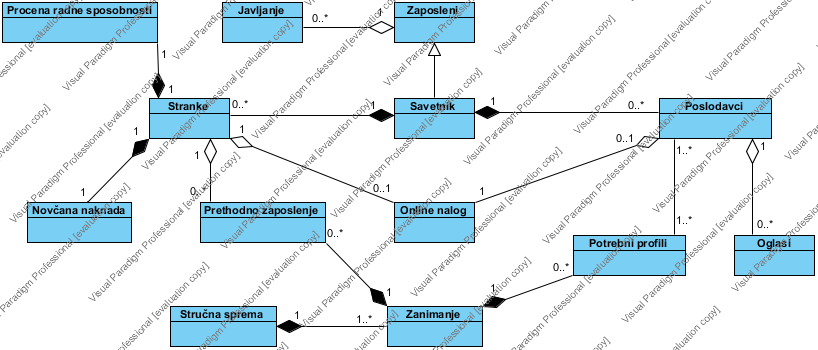
\includegraphics[width=0.85\paperwidth]{dijagrami/dijagrami-klasa/dijagrami-klasa.png}
	\caption{Dijagram klasa}
	\label{dk}
\end{figure}
\end{mylandscape}


\subsection{Podaci o zaposlenima u Nazcionalnoj slu\v zbi za zapo\v sljavanje}

Klasa "Zaposleni" sadr\v zi sve potrebne podatke o zaposlenima uklju\v cuju\' ci:
\begin{itemize}
	\item Ime i prezime
	\item JMBG
	\item Datum ro\dj enja
	\item Adresa stanovanja
	\item Telefon
	\item E-mail adresa
	\item Datum zaposlenja
	\item Pozicija (\v salterski slu\v zbenik, savetnik za zapo\v sljavanje, savetnik za poslodavce, administrator sistema)
	\item Plata
	\item \v Sifra (za logovanje na sistem)
\end{itemize}

\subsection{Podaci o nezaposlenim licima na evidenciji}

Klasa "Nezaposlena lica" sadr\v i li\v cne podatke o licu, kao i podatke o zanimanju stru\v cnoj spremi.
\\
\\ Podaci o nezaposlenim licima:
\begin{itemize}
	\item Ime i prezime
	\item Broj li\v cne karte
	\item JMBG
	\item Datum ro\dj enja
	\item Pol
	\item Mesto stanovanja
	\item Op\v stina stanovanja
	\item Adresa stanovanja
	\item Ku\' cni broj
	\item Broj stana 
	\item Datum prijave na evidenciju
	\item Telefon
	\item E-mail adresa
	\item Status (aktivan, zamrznut, zaposlen)
	\item Zaduzeni savetnik (referenca na Zaposleni)
	\item Procena radne sposobnosti
\end{itemize}

\noindent Podaci o prethodnim zaposlenjima:
\begin{itemize}
	\item Naziv
	\item Opis radnog mesta
\end{itemize}

\noindent Podaci o javljanju:
\begin{itemize}
	\item Datum javljanja
	\item Online (bool vrednost koja ozna\v cava da li je javljanje obavljeno putem interneta ili li\v cno u slu\v bi)
	\item Odlazak kod savetnika (bool vrednost koja ozna\v cava da li lice \v zeli da ode i kod savetnika)
	\item Termin za odlazak kod savetnika
	\item Datum zakazanog slede\' ceg javljanja
\end{itemize}

\noindent Podaci o nov\v canoj naknadi:
\begin{itemize}
	\item Prose\v cna zarada
	\item Broj ra\v cuna
	\item \v Sifra banke - po\v ste
\end{itemize}

\noindent Podaci o nalogu za online javljanje:
\begin{itemize}
	\item E-mail
	\item Lozinka
	\item ....
\end{itemize}

\noindent Podaci o proceni radne sposobnosti:
\begin{itemize}
	\item Ime i prezime lekara veštaka Republi\v ckog fonda penzijskog i invalidskog osiguranja
	\item Ime i prezime specijaliste medicine rada
	\item Ime i prezime psihologa
	\item Stru\v cni radnik Nacionalne slu\v zbe za zapo\v sljavanje (referenca na Zaposleni)
	\item Prostorija
	\item Datum i vreme
\end{itemize}


\subsection{Poslodavci}
Klasa Poslodavci obuhvata sve podatke o kompanijama koje \v zele da sara\dj uju sa Nacionalnom slu\v zbom za zaposljavanje kao i o njihovim potrebama i oglasima.
\\
\\ Podaci o kompaniji:
\begin{itemize}
	\item Naziv
	\item Opis
	\item Ime i prezime vlasnika
	\item Broj li\v cne katre vlasnika
	\item Adresa
	\item Telefon
	\item E-mail adresa
	\item Veb stranica
\end{itemize}

\noindent Podaci o oglasima i konkursima za poslove:
\begin{itemize}
	\item Opis radnog mesta
	\item Pla\' ceno
	\item Suma
	\item Odobreno (bool vrednost koja ozna\v cava da li je oglas odobren ili ne)
\end{itemize}

\noindent Podaci o potrebnim profilima ljudi:
\begin{itemize}
	\item Zvanje
	\item Stru\v cna sprema
	\item Broj otvorenih pozicija
\end{itemize}

\noindent Podaci o nalogu za online otvaranje oglasa:
\begin{itemize}
	\item E-mail adresa
	\item Lozinka
	\item ....
\end{itemize}


\subsection{Zanimanja}
Klasa "Zanimanja" odnosi se na podatke o stru\v cnoj spremi i zvanjima koja postoje.
\\
\\ Podaci o zvanjima:
\begin{itemize}
	\item Naziv
	\item Opis
	\item Stru\v cna sprema
\end{itemize}

\noindent Podaci o stru\v cnoj spremi:
\begin{itemize}
	\item Stepen
	\item Opis
	\item Godine za stepen
	\item Godine ukupno
\end{itemize}
